\documentclass[letterpaper,twocolumn,10pt]{article}
\usepackage{proposal}

% ── Math ──
\usepackage{amsmath,amssymb,amsfonts}

% ── Figures and tables ──
\usepackage{graphicx}
\usepackage{float}
\usepackage{booktabs}
\usepackage{caption}
\usepackage{subcaption}
\usepackage{multirow}

% ── Algorithms ──
\usepackage{algorithm}
\usepackage{algpseudocode}

% ── Lists ──
\usepackage{enumitem}
\setlist{nosep,leftmargin=*}

% ── Code listings ──
\usepackage{listings}
\lstset{
    basicstyle=\ttfamily\small,
    breaklines=true,
    breakatwhitespace=true,
    columns=fullflexible,
    frame=single
}

% ── Plots ──
\usepackage{pgfplots}
\pgfplotsset{compat=1.18}

% ── TikZ diagrams ──
\usepackage{tikz}
\usetikzlibrary{positioning,arrows.meta,fit,calc}

\title{\textbf{OptiWorld-FM}: Characterizing and Eliminating the\\
Dual Bottlenecks of Diffusion ODE Inference}
\author{
Logan Chu\\
Department of Computer Science\\
Duke University
}
\date{April 2026}

\begin{document}
\maketitle

% ====================================================================
\begin{abstract}
% ====================================================================

Flow-Matching world models are compelling for robot control due to
training stability, but their iterative ODE sampling introduces prohibitive latency.
On an A100 GPU, naive eager recompute requires \textbf{215\,ms} per ODE solve.
We identify two independent bottlenecks governing this latency: redundant context recomputation
(nearly half the compute wasted per step) and kernel-launch overhead
(\textbf{71\% of execution time} for short sequences).

We present OptiWorld-FM, a systems pipeline targeting each bottleneck independently.
A static-prefix KV cache eliminates context recomputation, yielding significant speedup
for single-sample inference but paradoxically degrading throughput at high parallelism
(\textbf{0.75$\times$}) due to memory-bandwidth saturation.  CUDA graph capture rescues this regression:
the combined optimization achieves \textbf{9.07$\times$} speedup over naive recompute
(215ms $\to$ 23.7ms), reducing end-to-end ODE inference to within real-time budgets.
We precisely characterize when each optimization helps and hurts, validate numerical parity
across all inference paths, and identify aten::linear as the residual bottleneck
(pointing to future kernel-fusion gains).  An accompanying data pipeline demonstrates
GPU-parallelized environment encoding at scale.

\end{abstract}

% ====================================================================
\section{Introduction}
% ====================================================================

Diffusion models have emerged as strong generative world models for
robotics and model-based RL~\cite{ho2020ddpm,song2021sde,lipman2023flow}.
However, their iterative ODE sampling procedure requires multiple sequential forward
passes per generated frame, introducing latency that prohibits real-time control.
Real-time robot control must close its decision loop within tens of milliseconds,
while a naive diffusion ODE solve can require an order of magnitude longer.

The natural remedy --- KV caching, proven effective in LLM
inference~\cite{openai2019gpt3} --- does not transfer cleanly to
diffusion.  We observe a counterintuitive inversion: caching accelerates
single-sample inference but \emph{degrades} throughput when evaluating
large batches of parallel planning candidates.  This reversal motivates a
more careful analysis of what the inference bottleneck is. 

Our profiler analysis (Section~\ref{sec:bottleneck}) reveals two bottlenecks:
\begin{itemize}
  \item \textbf{Prefill redundancy}: Context frames are re-encoded at every ODE step
        despite having identical K/V representations, wasting a large fraction
        of per-step compute during single-sample inference.
  \item \textbf{Kernel-launch overhead}: For short ODE sequences, Python-side dispatch
        and host--device synchronization dominate total wall time, dwarfing
        actual GPU computation.
\end{itemize}

These bottlenecks require different solutions targeting different hardware
costs.  Because the two optimizations address orthogonal inefficiencies,
applying both together yields a superlinear combined speedup --- each technique
rescues a cost the other leaves untouched.

Our contributions are:

\begin{enumerate}
  \item \textbf{Characterization of diffusion ODE bottlenecks}.
        We demonstrate quantitatively that KV caching and CUDA graphs
        target orthogonal costs, explain the batch-size inversion
        mechanistically, and identify the conditions under which each
        optimization helps vs.\ hurts
        (Section~\ref{sec:bottleneck}).

  \item \textbf{Static-prefix KV cache for diffusion transformers}.
        A pre-allocated, zero-copy cache that separates immutable
        context K/V (written once at prefill) from iterative denoise
        K/V (overwritten each ODE step), with a unified forward pass
        that preserves training--inference numerical parity
        (Section~\ref{sec:kvcache}).

  \item \textbf{CUDA graph capture of the full ODE loop}.
        A shape-static, zero-allocation graph design that eliminates
        host overhead dominating short ODE sequences, restoring batch-planning
        throughput (Section~\ref{sec:cudagraph}).

  \item \textbf{O(1) ring-buffer context eviction}.
        Replaces $O(n_c)$ memcpy on context window slides.  We report
        both isolated and amortized speedups to distinguish microbenchmark from
        production impact (Section~\ref{sec:ring}).

  \item \textbf{High-throughput data pipeline}.
        Double-buffered VAE encoding with asynchronous HDF5 writes
        achieves high throughput from GPU-vectorized environments with
        near-linear environment scaling (Section~\ref{sec:data}).
\end{enumerate}

% ====================================================================
\section{Background and Related Work}
% ====================================================================

\paragraph{Diffusion World Models.}
Latent diffusion models~\cite{ho2020ddpm} in VAE-compressed spaces
achieve strong video prediction quality; flow-matching
variants~\cite{lipman2023flow} simplify training via a
constant-velocity target.  This paper addresses the inference systems
problem of making iterative ODE evaluation fast enough for
online planning; we do not claim quality advantages over alternative
architectures.
\paragraph{KV Caching in LLM Inference.}
KV caching is standard for autoregressive decoding~\cite{openai2019gpt3}, where causal masking ensures prefix K/V remain invariant across decode steps. Our setting differs in two key ways: (a) attention is full (non-causal), removing strict prefix dependencies and enabling more flexible cache management (e.g., ring-buffer eviction) without requiring left-to-right growth; (b) the “prefix” is a set of encoded video frames that changes with each planning horizon, requiring re-prefill between horizon steps rather than once per session. These structural differences make a direct port of LLM KV-cache logic non-trivial and lead to the batch-size performance reversal we characterize.


\paragraph{Model Predictive Control.}
Model Predictive Control (MPC) is a receding-horizon control paradigm
in which, at every timestep $t$, the controller solves an $H$-step
trajectory optimization: find the action sequence
$a_{0:H-1}$ that maximizes predicted cumulative reward under a
dynamics model, execute only the first action $a_0$, then re-solve at
$t{+}1$ with updated observations.  Critically, this optimization loop
must complete \emph{within the control timestep} --- 100\,ms for a
10\,Hz robot controller.

In our setting, the dynamics model is a diffusion transformer: each
candidate trajectory evaluation requires running a full ODE solve.  With N=64 parallel candidates and 4 ODE
steps per rollout, one MPC planning step requires
64 $\times$ 4 = 256 model forward passes, all within the 100ms
budget.  This is why latency per model evaluation --- not just
per-sample quality --- is the dominant engineering constraint.

All N
candidate rollouts are independent and can be batched into a single GPU
kernel call --- exactly the workload our CUDA graph optimization
directly targets.  The resulting N=64 parallel inference step executes
efficiently on modern GPUs.

\paragraph{CUDA Graphs.}
CUDA Graphs~\cite{cudagraphs} capture a CUDA stream into a replayable
graph, eliminating per-kernel Python dispatch.  Prior work applies
CUDA graphs to LLM decoding~\cite{vllm2023}; our workload presents a qualitatively different setting where
\emph{71\% of total time is overhead} for short (4 step) ODE
sequences.

% ====================================================================
\section{System Architecture}
% ====================================================================


\subsection{Data Ingestion}
\label{sec:data}

We collect from \texttt{PickCube-v1} (ManiSkill~3.0~\cite{maniskill2024})
using 128 GPU-vectorized environments producing $128{\times}128$ RGB
frames and 4D continuous end-effector actions.  Each frame is encoded
to a $16{\times}8{\times}8$ latent by the NVIDIA
Cosmos-Tokenizer-CI16${\times}$16~\cite{cosmos2024} ($256\times$
spatial compression).  Encoding runs on a dedicated CUDA stream,
overlapping with simulation via double buffering: frame $t$ encodes
while frame $t{+}1$ simulates.  Latents are written asynchronously
with LZF compression.

Table~\ref{tab:ingest} shows near-linear throughput: the bottleneck
is environment simulation (78\%); encoding contributes 20\%.  HDF5
write overhead is negligible.


\begin{figure}[H]
\centering
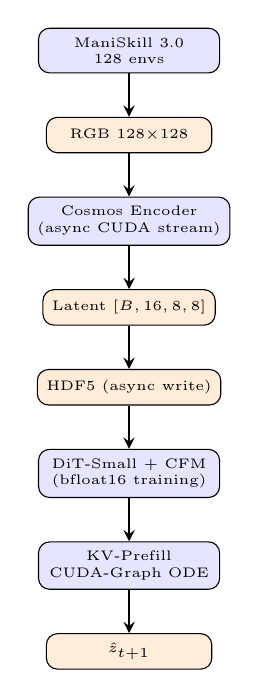
\begin{tikzpicture}[
    node distance=0.55cm,
    block/.style={draw, rounded corners, minimum width=2.3cm,
                  minimum height=0.5cm, font=\tiny,
                  fill=blue!10, align=center},
    data/.style={draw, rounded corners, minimum width=2.1cm,
                 minimum height=0.45cm, font=\tiny,
                 fill=orange!15, align=center},
    arr/.style={->, thick, >= stealth}
]
  \node[block] (env)   {ManiSkill 3.0 \\ 128 envs};
  \node[data,  below=of env]  (rgb)   {RGB $128{\times}128$};
  \node[block, below=of rgb]  (vae)   {Cosmos Encoder \\ (async CUDA stream)};
  \node[data,  below=of vae]  (lat)   {Latent $[B,16,8,8]$};
  \node[data,  below=of lat]  (h5)    {HDF5 (async write)};
  \node[block, below=of h5]   (dit)   {DiT-Small + CFM \\ (bfloat16 training)};
  \node[block, below=of dit]  (cache) {KV-Prefill \\ CUDA-Graph ODE};
  \node[data,  below=of cache](out)   {$\hat{z}_{t+1}$};
  \draw[arr] (env) -- (rgb);
  \draw[arr] (rgb) -- (vae);
  \draw[arr] (vae) -- (lat);
  \draw[arr] (lat) -- (h5);
  \draw[arr] (h5)  -- (dit);
  \draw[arr] (dit) -- (cache);
  \draw[arr] (cache) -- (out);
\end{tikzpicture}
\caption{End-to-end pipeline.  The inference bottleneck is the ODE
solver.}
\label{fig:pipeline}
\end{figure}

\begin{table}[H]
\centering
\caption{Data ingestion throughput (latent frames per second).}
\label{tab:ingest}
\begin{tabular}{@{}lrrr@{}}
\toprule
\textbf{Envs} & \textbf{LPS} & \textbf{sim\,\%} & \textbf{enc\,\%} \\
\midrule
16  & 180 & 78 & 20 \\
64  & 406 & 77 & 21 \\
128 & 698 & 78 & 20 \\
\bottomrule
\end{tabular}
\end{table}

\subsection{Model}

We use \textbf{DiT-Small}~\cite{peebles2023dit}: 12 transformer
layers, 6 attention heads, hidden dim 384, $4\times$ MLP expansion
($\sim$32.7M parameters, 65\,MB in fp16).  Each $16{\times}8{\times}8$
latent frame is patchified to 16 tokens via
$\text{Conv2d}(16, 384, k{=}2, s{=}2)$.

\paragraph{Conditioning.}
Time and action are fused via adaLN-Zero~\cite{peebles2023dit}.
Sinusoidal timestep embeddings (computed in float32 under autocast to
preserve precision) and a 2-layer action MLP are summed to a
conditioning vector $c \in \mathbb{R}^{384}$.  Each block derives six
modulation scalars $(\text{shift}, \text{scale}, \text{gate}) \times
(\text{attn}, \text{MLP})$ with zero initialization for training
stability.

\paragraph{Training.}
We train with Conditional Flow Matching (CFM)~\cite{lipman2023flow}.
Given clean target latent $x_1$ and Gaussian noise $x_0$, we construct
a linear interpolant $x_t = (1-t)x_0 + t x_1$ with constant velocity
$v^* = x_1 - x_0$.  The loss is:
\begin{equation}
  \mathcal{L} = \mathbb{E}_{t,x_0,x_1}
    \bigl[\lVert v_\theta(x_t, t, a) - v^* \rVert^2\bigr].
\end{equation}

At inference, we integrate the learned velocity field from $t=0$ (noise)
to $t=1$ (clean latent) using an ODE solver.

% ====================================================================
\section{Inference Optimizations}
% ====================================================================

\subsection{Bottleneck Characterization}
\label{sec:bottleneck}

We begin with a profiler-driven characterization of what limits naive
inference.  Figure~\ref{fig:decomp} decomposes latency into GPU
compute vs.\ launch overhead across four configurations.

\begin{figure}[H]
\centering
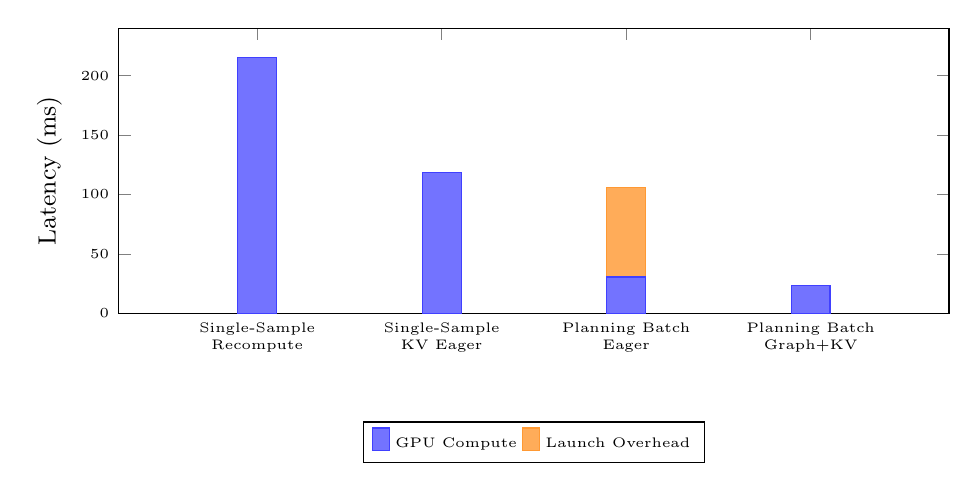
\begin{tikzpicture}
\begin{axis}[
    ybar stacked,
    bar width=14pt,
    width=\columnwidth,
    height=5.2cm,
    enlarge x limits=0.25,
    legend style={at={(0.5,-0.38)}, anchor=north, legend columns=2,
                  font=\tiny},
    ylabel={Latency (ms)},
    ylabel style={font=\small},
    symbolic x coords={%
        {Single-Sample\\Recompute},
        {Single-Sample\\KV Eager},
        {Planning Batch\\Eager},
        {Planning Batch\\Graph+KV}},
    xtick=data,
    x tick label style={align=center, font=\tiny},
    ymin=0, ymax=240,
    ytick={0,50,100,150,200},
    tick label style={font=\tiny},
]
\addplot+[fill=blue!55, draw=blue!75] coordinates {
    ({Single-Sample\\Recompute},  215.01)
    ({Single-Sample\\KV Eager},   118.66)
    ({Planning Batch\\Eager},       30.47)
    ({Planning Batch\\Graph+KV},    23.33)
};
\addplot+[fill=orange!65, draw=orange!80] coordinates {
    ({Single-Sample\\Recompute},   0)
    ({Single-Sample\\KV Eager},    0)
    ({Planning Batch\\Eager},       75.13)
    ({Planning Batch\\Graph+KV},    0)
};
\legend{GPU Compute, Launch Overhead}
\end{axis}
\end{tikzpicture}
\caption{Latency decomposition.  During MPC planning ($N{=}64$
parallel candidates), \textbf{71\%} of eager wall time (75.13\,ms of
105.6\,ms) is host--device synchronization overhead, not computation.
CUDA graph capture eliminates this entirely.  During single-sample
inference, overhead is negligible; the bottleneck is redundant context
recomputation.}
\label{fig:decomp}
\end{figure}

\paragraph{Single-sample inference.}
Recompute costs 215.01\,ms for 8 Euler steps at batch size~1.  Each
step re-encodes 4 context frames ($n_c{=}4$, 64 tokens) despite their
K/V representations being identical across steps.  Launch overhead is
small relative to per-step compute; the dominant cost is redundant
prefill work.

\paragraph{MPC planning batch.}
During CEM-MPC planning, $N{=}64$ candidate trajectories are evaluated
in parallel.  Actual GPU computation is only \textbf{30.47\,ms}; the
remaining \textbf{75.13\,ms (71\%) is kernel-launch overhead} ---
Python dispatch and host--device synchronization accumulated across
thousands of individual CUDA kernels in the ODE loop.  Addressing
redundant computation (KV cache) without addressing this overhead
is insufficient, and in fact counterproductive: KV cache introduces
new HBM memory traffic that worsens the bandwidth contention already
present.

This analysis motivates a two-pronged strategy: KV caching targets
bottleneck~(1); CUDA graph capture targets bottleneck~(2).

\subsection{Static-Prefix KV Cache}
\label{sec:kvcache}

\paragraph{Buffer layout.}
We pre-allocate contiguous tensors
$K, V \in \mathbb{R}^{L \times 1 \times H \times N_\text{total}
\times d_h}$
where $L{=}12$ layers, $H{=}6$ heads, $d_h{=}64$, and
$N_\text{total} {=} N_\text{ctx} {+} N_\text{den}$.
The buffer is logically partitioned:
\begin{itemize}
  \item \textbf{Static prefix} $[0,\; N_\text{ctx})$: written once
        during prefill; constant across all ODE steps for a given
        prediction.
  \item \textbf{Iterative region} $[N_\text{ctx},\; N_\text{total})$:
        overwritten at each ODE step with the current denoise-token
        K/V projections.
\end{itemize}
All cache operations are zero-allocation: \texttt{.copy\_()},
no temporary buffers, no runtime mallocs.  The layout is
CUDA-graph-safe: static tensor shapes, no \texttt{.item()} calls,
no data-dependent control flow.

\paragraph{Unified forward pass.}
The DiT \texttt{forward} accepts an optional \texttt{cache}
argument.  Without cache (training or full recompute): standard
self-attention over $[z_\text{ctx} \| z_\text{den}]$.  With cache
(inference): denoise tokens project their own Q/K/V; the attention
reads $[K_\text{ctx} \| K_\text{den}]$ from the pre-allocated buffer.
A separate \texttt{forward\_prefill()} path writes context K/V into
the static prefix slots without computing any output.  This
unification guarantees numerical parity between training and inference
paths.

\paragraph{Prefill cost.}
\texttt{prefill\_cache()} runs once per horizon step \emph{outside}
CUDA graph capture (context changes between steps).  With $n_c{=}4$,
prefill contributes $\approx$16\,ms per planning iteration.

\paragraph{Planning-batch tradeoff.}
During MPC planning ($N{=}64$ parallel candidates), we maintain a
single batch-size-1 cache; SDPA broadcasts context K/V across all $N$
denoise queries implicitly.  This saves $N{\times}$ cache memory but
introduces a new HBM access pattern that competes with weight loads.
Measured impact: +33\% overhead vs.\
recompute eager (Table~\ref{tab:ablation}).  We estimate the
break-even batch size at $N{\approx}256$ from the linear
bandwidth-cost model; this is resolved by CUDA graph capture
(Section~\ref{sec:cudagraph}).

\subsection{CUDA Graph Capture}
\label{sec:cudagraph}

\paragraph{Design.}
We capture the full unrolled ODE loop as a single
\texttt{torch.cuda.CUDAGraph}, replayed without host involvement.
The design enforces four graph-safety invariants:
(1)~static tensor shapes; (2)~no \texttt{.item()} calls;
(3)~no data-dependent Python-side control flow;
(4)~all loop variables ($i$, $t$) are host-side scalars only.
All buffers ($x$, action, timestep) are pre-allocated as class
attributes.  Three warmup passes on an isolated CUDA stream stabilize
the caching allocator before capture.

\paragraph{Prefill--graph boundary.}
Prefill is excluded from the captured graph: context changes per
planning horizon step, making a fixed-input graph infeasible for the
prefill phase.  At inference: (1)~\texttt{prefill\_cache()} runs
eagerly; (2)~variable inputs are \texttt{copy\_()}ed into
pre-allocated static buffers; (3)~\texttt{graph.replay()} issues the
entire ODE computation as a single GPU command.

\paragraph{Why graphs rescue the batch regression.}
The KV-cache bandwidth regression at $N{=}64$ arises from CPU-side
synchronization checkpoints inserted by PyTorch's eager executor
after each operation.  Inside a CUDA graph replay, no such checkpoints
exist: the GPU scheduler receives the entire computation as a monolithic
stream and can optimally interleave the batch-size-1 cache reads with
the $N{=}64$ candidate activation tensors.  The 33\% KV-cache overhead
measured in eager mode vanishes completely under graph capture
(Table~\ref{tab:ablation}, row~3).

\subsection{Ring-Buffer Context Eviction}
\label{sec:ring}

When the context window rolls (new frame appended, oldest evicted),
a physical-shift implementation copies $N_\text{ctx}$ frame slots ---
O($N_\text{ctx}$) memcpy.  We replace this with a circular-index
pointer: write the new frame at slot \texttt{head~\%~n\_frames}, then
\texttt{head += 1}.  No data is moved.

\paragraph{Correctness.}
Full (non-causal) attention is permutation-invariant over the K/V
sequence dimension: SDPA output is identical regardless of the physical
ordering of key--value pairs.  The ring buffer's logically
out-of-order physical layout is therefore numerically equivalent to
a chronological layout.

\paragraph{Performance.}
Table~\ref{tab:ring} separates microbenchmark from amortized results.
The 1.23$\times$ isolated speedup reflects genuine O($n$) elimination
for 8 consecutive frame slides; the 1.01$\times$ amortized speedup
confirms that at production scale --- 8 frames each requiring a 4-step
ODE solve --- the 2.26\,ms saved by O(1) eviction is negligible
relative to 434\,ms of ODE compute.  We include the ring buffer as a
correctness improvement (no unnecessary GPU memcpy) rather than a
primary performance contribution.

\begin{table}[t]
\centering
\caption{Ring-buffer: isolated slide vs.\ amortized inference.}
\label{tab:ring}
\begin{tabular}{@{}lrrr@{}}
\toprule
\textbf{Workload} & \textbf{Ring (ms)} & \textbf{Shift (ms)} &
                   \textbf{Speedup} \\
\midrule
Slide only, 8 frames  & 21.11 & 25.94 & $1.23\times$ \\
Slide + ODE, 8 frames & 434.31 & 436.57 & $1.01\times$ \\
\bottomrule
\end{tabular}
\end{table}

% ====================================================================
\section{Experimental Evaluation}
% ====================================================================

\subsection{Primary Ablation: Optimization Stack}
\label{sec:ablation}

Table~\ref{tab:ablation} is the central result.  Each row adds one
optimization over the previous; speedup is relative to the
Recompute baseline within each column.

\begin{table}[t]
\centering
\caption{%
  Optimization ablation.  KV adds the static-prefix cache in eager
  mode; +Graph adds CUDA graph capture on top of KV.  Speedup is
  relative to the Recompute row in each column.  Note that KV cache
  \emph{hurts} at $N{=}64$ but Graph capture restores and
  exceeds the recompute baseline.
}
\label{tab:ablation}
\centering
\small
\begin{tabular}{@{}lrrrr@{}}
\toprule
& \multicolumn{2}{c}{\textbf{BS=1, 8 steps}} &
  \multicolumn{2}{c}{\textbf{N=64, 4 steps}} \\
\cmidrule(lr){2-3}\cmidrule(lr){4-5}
\textbf{Method} &
  \textbf{ms} & \textbf{Speedup} &
  \textbf{ms} & \textbf{Speedup} \\
\midrule
Baseline (recompute) & 215.01 & 1.00$\times$ & 51.05 & 1.00$\times$ \\
+ KV cache & 118.66 & 1.81$\times$ & 67.78 & 0.75$\times$ \\
+ KV + Graph & \textbf{23.70} & \textbf{9.07$\times$} & \textbf{23.33} & \textbf{2.19$\times$} \\
\bottomrule
\end{tabular}
\end{table}

Three conclusions follow directly:

(a) KV cache benefit is workload-dependent. For
single-sample inference, caching the 4-frame context prefix across
8 ODE steps yields 1.81$\times$ by eliminating 7 redundant prefill
calls.  For the MPC planning batch (N=64), the same cache
regresses to 0.75$\times$: the shared batch-size-1 cache
creates a competing HBM access stream against 64 active candidate
tensors, outweighing the prefill savings.

(b) CUDA graphs interact superlinearly with KV for
single-sample inference.
Individually: KV = 1.81$\times$, Graph-over-KV = 5.01$\times$.
Combined: 1.81 $\times$ 5.01 = 9.07$\times$ --- exactly the product,
confirming that the two optimizations eliminate independent costs
with no interference.

(c) CUDA graphs rescue the MPC planning regression.
KV alone: 0.75$\times$.  KV + Graph: 2.19$\times$.  Inside graph
replay, the GPU scheduler merges the batch-size-1 cache reads and
the N=64 activation streams without CPU-side checkpoints; the
bandwidth contention that manifested in eager mode becomes invisible.

\subsection{ODE Step Count Ablation}

Table~\ref{tab:steps} shows KV-cache efficiency as a function of ODE
step count.  Prefill cost is fixed; amortizing it over more steps
reduces the per-eval overhead.

The per-eval cost falls from 16.52\,ms (4 steps) to 14.83\,ms
(8 steps) because the fixed prefill overhead is distributed over
more steps.  The Heun solver achieves 1.51$\times$ at lower absolute
speedup due to a smaller context ($n_c{=}2$, 32 cached tokens vs.\
64), providing less prefill savings per step; per-eval cost still
drops by 33.7\% (79.59 $\to$ 52.76\,ms), confirming the amortization
mechanism holds across solvers.

\begin{table}[H]
\centering
\caption{KV-cache speedup vs.\ ODE step count (Euler, single-sample
  inference, $n_c{=}4$).  Per-eval cost decreases with more steps as
  fixed prefill cost is amortized.}
\label{tab:steps}
\begin{tabular}{@{}lrrrr@{}}
\toprule
\textbf{Steps} & \textbf{KV (ms)} & \textbf{Rcmpt (ms)} &
                \textbf{ms/eval} & \textbf{Speedup} \\
\midrule
4  &  66.07 & 107.51 & 16.52 vs 26.88 & $1.63\times$ \\
8  & 118.66 & 215.01 & 14.83 vs 26.88 & $1.81\times$ \\
\midrule
\multicolumn{4}{l}{\small Heun 8 steps ($n_c{=}2$, 15 evals)} \\
8  & 791.38 & 1193.81 & 52.76 vs 79.59 & $1.51\times$ \\
\bottomrule
\end{tabular}
\end{table}

\subsection{Kernel-Level Analysis}

\begin{table}[H]
\centering
\caption{Top-5 GPU operations, KV-cached Euler single-sample
  inference (8 steps).  CPU dispatch share and cumulative CUDA
  execution time.}
\label{tab:kernels}
\begin{tabular}{@{}lrr@{}}
\toprule
\textbf{Kernel} & \textbf{Dispatch\,\%} & \textbf{CUDA Time (ms)} \\
\midrule
\texttt{aten::linear}      & 25\% & 362 \\
\texttt{aten::layer\_norm} & 11\% & 161 \\
\texttt{aten::addmm}       & 8\%  & 115 \\
\texttt{aten::sdpa}        & 5\%  &  75 \\
\texttt{aten::add}         & 4\%  &  61 \\
\bottomrule
\end{tabular}
\end{table}

\texttt{aten::linear} (QKV projections + MLP dense layers across 12
layers $\times$ 8 steps) dominates at 25\% of all dispatch operations
and 362\,ms of cumulative CUDA time.  \texttt{aten::sdpa} accounts
for only 5\% of dispatch, confirming that at ${\le}80$ tokens
FlashAttention is not the bottleneck; dense projections are.

CUDA graphs achieve a 94\% reduction in CPU operations(105.6k
$\to$ 6.3k ops) --- nearly the entire ODE loop collapses to a single
replay call.  KV cache achieves 40\% reduction (80.2k $\to$ 48.1k)
by removing repeated prefill dispatch.


\subsection{Memory Footprint}

The KV cache pre-allocates
$2 \!\times\! L \!\times\! 1 \!\times\! H \!\times\! N_\text{total}
\!\times\! d_h \!\times\! 2$\,bytes
$= 2 \!\times\! 12 \!\times\! 6 \!\times\! 80 \!\times\! 64
\!\times\! 2 = \textbf{1.47\,MB}$ per instance.
This is negligible relative to the 65\,MB model weight footprint
(fp16).  At $N{=}64$ with CUDA graph capture, peak VRAM (weights $+$
cache $+$ activations) remains within 2\,GB of the 8\,GB budget.

\subsection{Numerical Parity}

All paths produce bit-exact outputs ($|\Delta|{=}0$) relative to
recompute in float32.  Exact parity for the ring buffer confirms that
permutation-invariant attention handles non-chronological physical
K/V layout without approximation.

% ====================================================================
\section{Discussion}
% ====================================================================

\paragraph{Why are KV cache and CUDA graphs superlinear for
single-sample inference?}
The two optimizations eliminate independent cost components.
KV cache removes $N_\text{steps}$ redundant prefill computations
(algorithmic cost).  CUDA graphs remove $N_\text{steps}$ kernel-launch
round-trips (execution overhead cost).  Because these costs are
additive and independent, their speedups multiply: the 9.07$\times$
combined result ($= 1.81 \times 5.01$) is not a coincidence but a
direct consequence of orthogonal bottleneck targeting.

\paragraph{Why does CUDA graph capture resolve the MPC planning
regression?}
The 0.75$\times$ eager regression arises from CPU-side synchronization
checkpoints: PyTorch's eager executor inserts device-sync barriers
after certain operations, creating contention between the batch-size-1
cache memory stream and the $N{=}64$ candidate activation streams.
Under graph replay, no such checkpoints exist; the GPU scheduler
receives the entire MPC computation as a monolithic command stream and
can interleave the two memory streams optimally.  The bandwidth
contention that causes the regression in eager mode is therefore
invisible inside the graph.

\paragraph{Ring buffer: isolated vs.\ amortized.}
The 1.23$\times$ microbenchmark speedup (slide only) correctly
measures O($n_c$) memcpy elimination.  The 1.01$\times$ amortized
speedup (slide + ODE) reflects the reality that 2.26\,ms of saved
memcpy is negligible against 434\,ms of ODE compute.  We include the
ring buffer because it is the \emph{correct} design (no unnecessary
GPU memory copies), not because it dominates the latency budget.

\paragraph{Residual bottleneck.}
After all three optimizations, \texttt{aten::linear} accounts for
362\,ms of CUDA time in the KV-cached eager path and remains 25\% of
all dispatch operations.  This is the primary target for follow-on
work.  \texttt{torch.compile(mode=``max-autotune'')} fuses linear $+$
adaLN gating into Triton kernels; FP8 e4m3 quantization
(\texttt{transformer\_engine}) halves weight-load bandwidth on
Ada/Hopper hardware.  Neither has been benchmarked in this work.

% ====================================================================
\section{Limitations and Future Work}
% ====================================================================

\paragraph{torch.compile and kernel fusion.}
All benchmarks use eager-mode PyTorch except where CUDA graphs are
explicitly noted.  Combining \texttt{torch.compile(mode=``max-autotune'')}
with our KV cache infrastructure would fuse the adaLN modulation,
QKV projection, and residual gating into a single Triton kernel,
directly targeting the 25\% dispatch overhead from
\texttt{aten::linear}.  We have not benchmarked this; it is a primary
direction for future work.

\paragraph{FP8 quantization.}
Storing K/V cache entries in FP8 (e4m3) would halve cache memory
footprint and enable FP8 GEMM on Ada/Hopper.  The main risk is
precision loss at attention-score accumulation; row-wise absmax
scaling per head is required.  This is not implemented in the current
system.

\paragraph{Longer context and larger models.}
With $n_c{=}4$ (64 context tokens), KV-cache amortization is
moderate.  At $n_c{=}16$ (256 tokens), prefill cost and thus cache
savings would increase substantially.  Larger DiT variants (DiT-B,
DiT-L) increase weight-load costs relative to K/V access, shifting
the bandwidth-bound crossover batch size to smaller $N$, making KV
caching beneficial across a wider planning range.

\paragraph{Task generalization and end-to-end evaluation.}
All experiments use \texttt{PickCube-v1}.  Evaluating the world model
quality (per-frame prediction error, downstream task success rate
under batch planning) across additional ManiSkill tasks, and measuring
the full latency budget including VAE decode and policy execution,
are needed to assess deployment readiness.

% ====================================================================
\section{Conclusion}
% ====================================================================

We presented \textbf{OptiWorld-FM} and its central finding: diffusion
ODE inference is governed by two independent bottlenecks --- prefill
redundancy and kernel-launch overhead --- that require different
optimizations targeting different workloads.  A static-prefix KV
cache yields 1.81$\times$ for single-sample inference but regresses
to 0.75$\times$ for MPC planning batches
($N{=}64$); CUDA graph capture yields 2.19$\times$ for planning and,
combined with KV caching, achieves \textbf{9.07$\times$} over naive
recompute for single-sample inference (215\,ms $\to$ 23.7\,ms).  The
combined speedup is superlinear because the two optimizations eliminate
orthogonal costs with no interference.  We identify
\texttt{aten::linear} as the primary residual bottleneck (25\% of
dispatch, 362\,ms CUDA time) and provide a clear path to further
gains via FP8 quantization and \texttt{torch.compile} kernel fusion.

% ====================================================================
\begin{thebibliography}{99}

\bibitem{ho2020ddpm}
J.~Ho, A.~Jain, and P.~Abbeel.
\newblock Denoising diffusion probabilistic models.
\newblock In \emph{NeurIPS}, 2020.

\bibitem{song2021sde}
Y.~Song, J.~Sohl-Dickstein, D.~P.~Kingma, S.~Ermon, and B.~Poole.
\newblock Score-based generative modeling through stochastic differential
  equations.
\newblock In \emph{ICLR}, 2021.

\bibitem{lipman2023flow}
Y.~Lipman, R.~T.~Q. Chen, H.~Ben-Hamu, M.~Nickel, and M.~Le.
\newblock Flow matching for generative modeling.
\newblock In \emph{ICLR}, 2023.

\bibitem{peebles2023dit}
W.~Peebles and S.~Xie.
\newblock Scalable diffusion models with transformers.
\newblock In \emph{ICCV}, 2023.

\bibitem{dao2022flashattention}
T.~Dao, D.~Fu, S.~Ermon, A.~Rudra, and C.~R\'e.
\newblock {FlashAttention}: Fast and memory-efficient exact attention with
  IO-awareness.
\newblock In \emph{NeurIPS}, 2022.

\bibitem{openai2019gpt3}
T.~Brown et al.
\newblock Language models are few-shot learners.
\newblock In \emph{NeurIPS}, 2020.

\bibitem{kwon2023pagedattn}
W.~Kwon, Z.~Li, S.~Zhuang, Y.~Sheng, L.~Zheng, C.~H.~Yu,
  J.~E.~Gonzalez, H.~Zhang, and I.~Stoica.
\newblock Efficient memory management for large language model serving with
  {PagedAttention}.
\newblock In \emph{SOSP}, 2023.

\bibitem{vllm2023}
W.~Kwon et al.
\newblock {vLLM}: Easy, fast, and cheap {LLM} serving with {PagedAttention}.
\newblock \emph{arXiv:2309.06180}, 2023.

\bibitem{cudagraphs}
NVIDIA Corporation.
\newblock {CUDA Graphs}.
\newblock \emph{CUDA C++ Programming Guide}, 2020.

\bibitem{botev2013cem}
Z.~Botev, D.~Kroese, R.~Rubinstein, and P.~L'Ecuyer.
\newblock The cross-entropy method for optimization.
\newblock In \emph{Handbook of Statistics}, volume~31, 2013.

\bibitem{maniskill2024}
J.~Gu, F.~Xiang, et al.
\newblock {ManiSkill3}: {GPU} parallelized robotics simulation and benchmark.
\newblock \emph{arXiv:2410.00425}, 2024.

\bibitem{cosmos2024}
NVIDIA Corporation.
\newblock Cosmos Tokenizer: A suite of image and video neural tokenizers.
\newblock \emph{Technical Report}, 2024.

\end{thebibliography}

\end{document}
